% !TeX root = ../../../thesis.tex

\section{DC Environment}
\label{sec:dc-environment}





In a DC environment, the code framework works well because the DC power signal is an easy signal to understand and work with.
For example, in \autoref{fig:dc-voltage-and-current-example} the voltage output of a DC power supply can be seen.
A load is switched on and off, and the current that flows over time can also be seen in the figure.
This switching causes the current to be a square wave with sharp edges.
The current is zero when the load is off and the current is a constant value for when the load is on.
This is the signal for one load.
If multiple of these current signatures will be aggregated, it will still be a square wave without distortions.

\begin{figure}[ht]
  \centering
  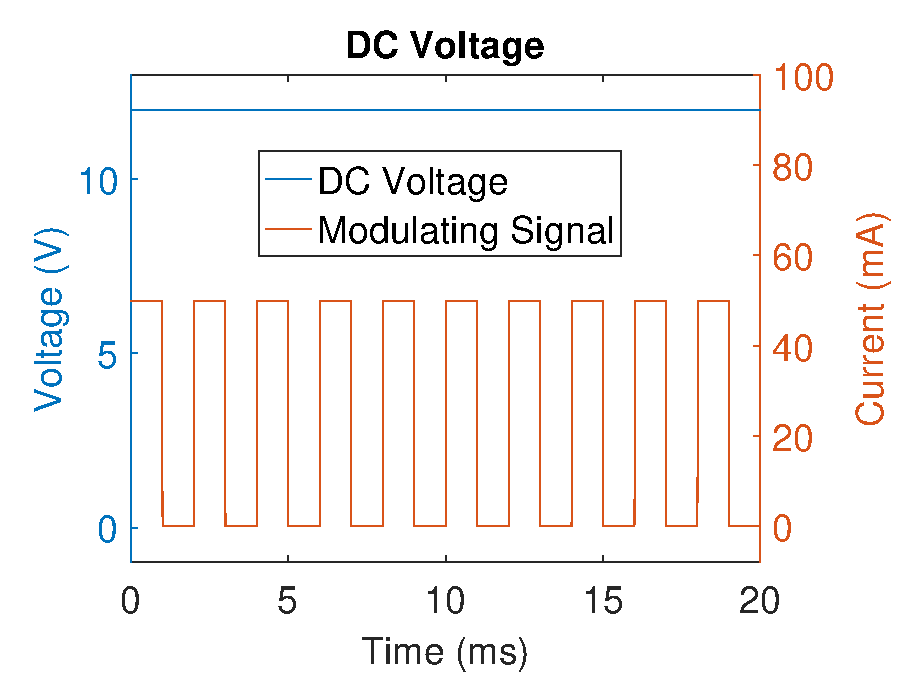
\includegraphics[angle=0,width=0.5\textwidth]{chapters/hardware-chapters/DC/dc-voltage-and-current-example.eps}
  \caption{Voltage of a DC power supply, along with the current of a switching load.}
  \label{fig:dc-voltage-and-current-example}
\end{figure}



This is the ideal way the modulator for an LED must work.
In the next sections, the hardware for the modulator will be explained as well as how the current will be measured to extract the encoded information and finally a testbed will be presented. 





% !TeX root = ../../../../thesis.tex

\subsection{Modulator}

	The task of the modulator is to switch the LED on or off based on the ID that is assigned to the light fixture.
	It is the responsibility of this piece of hardware to translate the ID into the unique current signature.


	The way an LED (Light Emitting Diode) works, is that current has to flow through it in order for it to emit light.
	In other words, an LED is controlled via current, it is not controlled by applying a voltage to it.
	When a certain amount of current flows through the LED, a certain amount of voltage will drop over the LED.

	The easiest way to make an LED emit light, is to put a current limiting resistor in series with a voltage source and an LED.
	A schematic can be seen in \autoref{fig:dc-led-resistor}.
	But there exists no ideal DC power supply.
	Depending on the load, the provided voltage of the power supply may fluctuate.
	Due to the fluctuation of the provided voltage, the LED can start to change in brightness.
	The current that flows through the LED is a function of the voltage over the resistor and the value of the resistor: $I = \frac{U}{R}$.
	So if $U$, the provided voltage, is fluctuating, the current that flows through the LED, $I$, will also fluctuate.
	This causes the brightness of the LED to fluctuate.


	A better way to power an LED, is by using a current source.
	Where an ideal voltage source will always deliver a certain amount of voltage independent of the load, a current source will always deliver a certain amount of current independent of the load.
	If a constant amount of current flows through the LED, the brightness will not fluctuate.
	In \autoref{fig:dc-led-current-source} a schematic can be seen, which shows an example of a current source powering an LED.
	This current source can be toggled on and off via a 0 V or 3.3/5 V signal, coming from a micro-controller, uC in the schematic.


	\begin{figure}[t]
		\centering
		\begin{minipage}[b]{0.3\textwidth}
			\includegraphics[width=\textwidth]{chapters/hardware-chapters/DC/dc-modulator/dc-led-resistor.jpg}
			\caption{Simplest way to power an LED.}
			\label{fig:dc-led-resistor}
		\end{minipage}
		\hfill
		\begin{minipage}[b]{0.5\textwidth}
			\includegraphics[width=\textwidth]{chapters/hardware-chapters/DC/dc-modulator/dc-led-current-source.jpg}
			\caption{Current source powering an LED.}
			\label{fig:dc-led-current-source}
		\end{minipage}
	\end{figure}

	By using a current source, two benefits can be identified:

	\begin{itemize}
		
		\item Since the current that flows through the LED is constant, the LED will not flicker.

		\item The current source will make sure that the current that is drawn, is either zero or some constant value depending on the bit that is being encoded.
		This will yield a signal with two distinct values.
		When multiple of these signals are aggregated and measured by a smart-meter, the measured signal will also have distinct values.
		This signal will make it easy to decode the information that was encoded by the modulators.

	\end{itemize}

% !TeX root = ../../../../thesis.tex

 \subsection{Current Sampler}

	Now that the hardware is created to translate the IDs of the LEDs into a unique current signature, we also need a way to measure the current.
	The measured current can then be processed by a micro-controller.
	And in turn it can be identified which LEDs are on and which are off.

	In the interest of time the most simple manner was chosen to measure the current for the DC hardware.
	Other options are available for measuring current and they will be discussed in the AC part.
	The most simple way to measure current is by using a series resistor.
	The resistance does not variate and therefor no noise is introduced in the sampled signal.
	The resistor is placed in series between the DC power supply and the LEDs.
	The voltage drop over the resistor is linearly proportional to the current that flows through the resistor, according to Ohm's Law $U = R \times I$.
	If the value of the resistor is chosen such that the maximum voltage will never exceed the rated voltage for a micro-controller, it can be directly measured by the micro-controller's ADC in question.

% !TeX root = ../../../../thesis.tex

\subsection{Testbed}
	\label{subsec:dc-testbed}

	To be able to test all aspects of the system a testbed was created.
	This testbed will allow the testing of the correlation calculations as discussed in \autoref{sec:mapping-problem}, the interference solutions (\autoref{subsec:continuous-method-modulation}), and the performance of the modulator and current-sampler.


	\begin{figure}[ht]
		\centering
		\includegraphics[angle=0,width=0.6\textwidth,height=.9\textheight,keepaspectratio]{chapters/hardware-chapters/DC/dc-test-bed/dc-test-bed-picture.JPG}
		\caption{Picture of the DC testbed, showing the six LED strips, current sources, current sampler and an Arduino board.}
		\label{fig:dc-test-bed-picture}
	\end{figure}

	\begin{figure}[ht]
		\centering
		\includegraphics[angle=0,width=1.0\textwidth,keepaspectratio]{chapters/hardware-chapters/DC/dc-test-bed/dc-test-bed-architectural.JPG}
		\caption{Architectural overview of the DC testbed. Six LED modulators are connected in parallel with each other and in series with the current sampler.}
		\label{fig:dc-test-bed-architectural}
	\end{figure}


	The testbed works with a DC power supply and has six individual controllable current sources.
	Each current source powers one LED fixture.
	The testbed itself can be seen in \autoref{fig:dc-test-bed-picture} and an architectural overview of how everything is connected to each other can be seen in \autoref{fig:dc-test-bed-architectural}.


	The aim of the testbed was to use commercial LEDs. 
	The LED fixtures used in this testbed all came from the same commercial LED, which can be found in \cite{commercial-230v-ac-led-aliexpress}.
	A picture of the LED can be seen in \autoref{fig:ac-commercial-230v-ac-led}.
	The strips are taken out of this commercial LED and used individually for this testbed.


	The current is measured by a series resistor and fed to the ADC of a micro-controller.
	The entire schematic of the DC testbed can be found in \autoref{app:dc-test-bed}. 

	The current sources and therefore the LEDs, can be toggled on and off by a micro-controller.
	By toggling the current sources on and off, the current that flows through the series resistor will change accordingly.
	A change of voltage over the series resistor can then be measured by the ADC.

	The measured current from the DC testbed can be seen in \autoref{fig:raw-dc-test-bed-data-short}.
	In this experiment, all six LEDs are modulating with the unique ID that was assigned to each LED.
	The voltage drop over the resistor is measured with the ADC.
	The raw ADC value can be seen on the left y-axis and the calculated aggregated current that is drawn can be seen on the right y-axis.
	From this figure seven distinguishable states can be seen.
	When there are no LEDs on, all LEDs are encoding a `0' data bit, the current is zero.
	When one of the six LEDs is transmitting a `1' data bit, the current jumps to roughly 50 mA.
	When two of the six LEDs are encoding a `1', the current is roughly 100 mA and so on.


	\begin{figure}
		\centering
		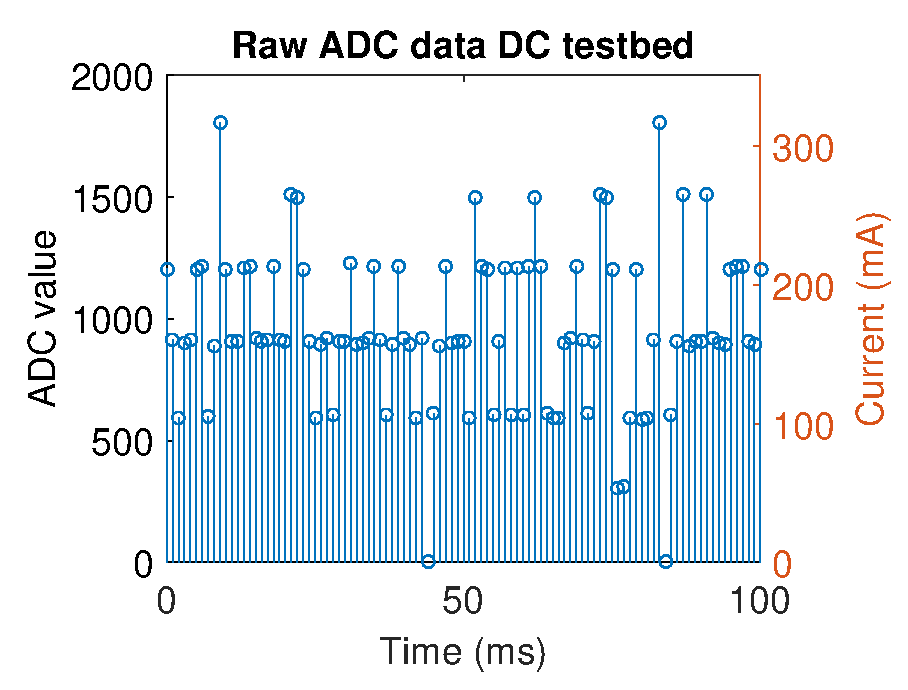
\includegraphics[angle=0,width=0.7\textwidth,keepaspectratio]{chapters/hardware-chapters/DC/dc-test-bed/dc-test-bed-raw-data.eps}
		\caption{Raw current data from the DC testbed with the six LEDs modulating with their unique IDs.}
		\label{fig:raw-dc-test-bed-data-short}
	\end{figure}



	An evaluation of this testbed is done in \autoref{subsec:dc-testbed-eval} where a longer signal will be shown along with correlation data to identify if a certain LED is on, while the other LEDs are modulating and thereby causing interference.











